\chapter{Thiết kế UML}
Các sơ đồ dưới đây là mô hình thiết kế đề xuất, dùng để thống nhất phạm vi và luồng xử lý trước implementation.
\section{Sơ đồ Usecase}
Use Case trả lời câu hỏi: ai sử dụng hệ thống và họ thực hiện chức năng gì?
\begin{figure}[H]\centering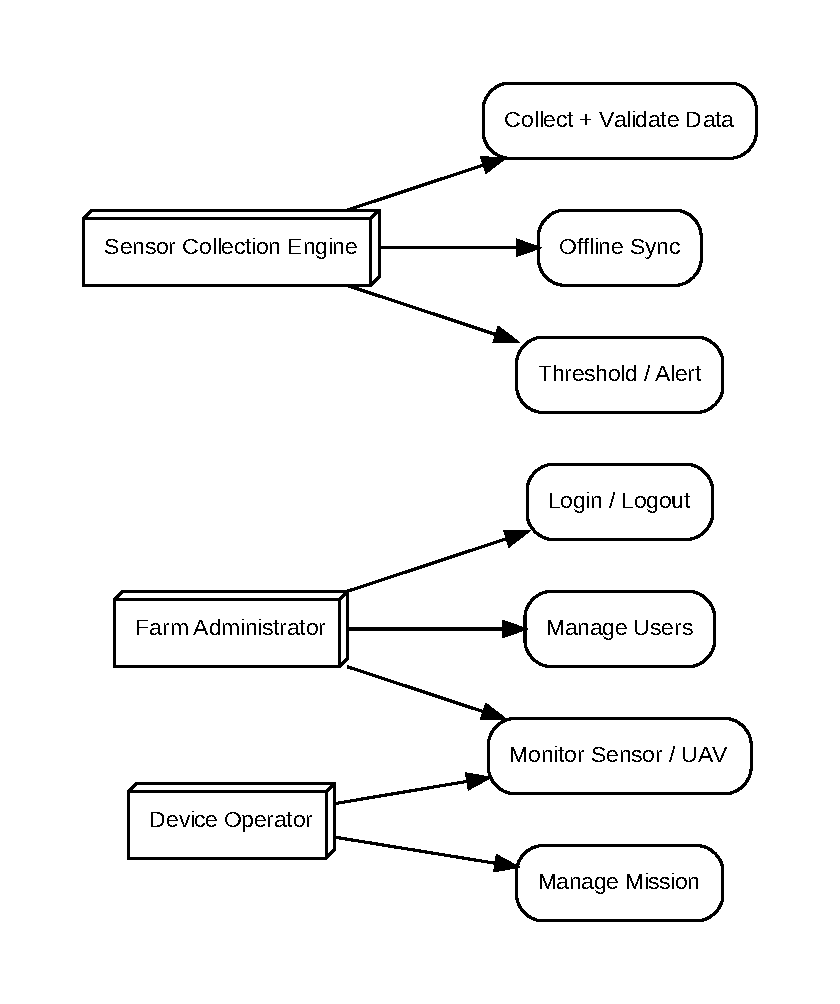
\includegraphics[width=0.95\textwidth,height=0.62\textheight,keepaspectratio]{diagrams/usecase.pdf}\caption{Use Case Diagram tổng quát}\end{figure}
\section{Class}
Class Diagram mô tả các entity miền nghiệp vụ chính và quan hệ của chúng.
\begin{figure}[H]\centering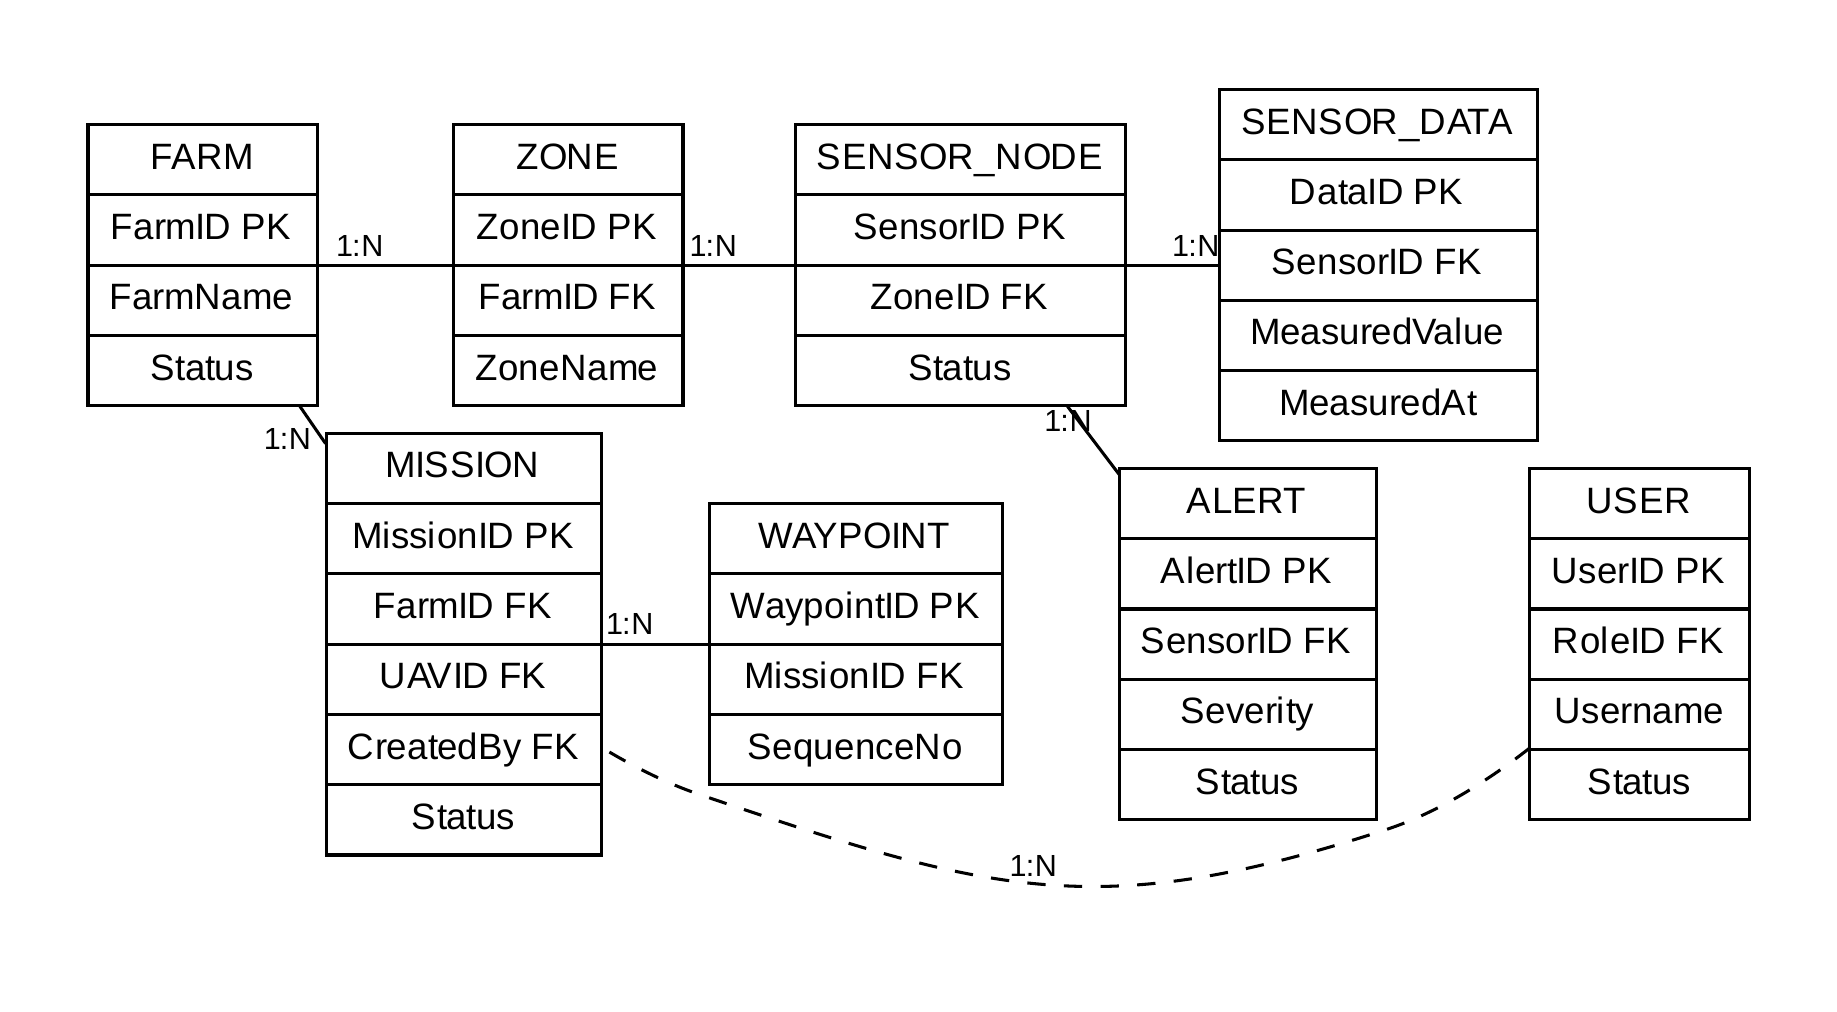
\includegraphics[width=0.95\textwidth,height=0.65\textheight,keepaspectratio]{diagrams/class.png}\caption{Class Diagram mức miền nghiệp vụ}\end{figure}
\section{Sơ đồ Activity}
Activity Diagram mô tả quy trình xử lý một measurement.